\documentclass[12pt, titlepage]{article}
\usepackage{graphicx}
\usepackage{booktabs}
\usepackage{tabularx}
\usepackage{longtable}
\usepackage{hyperref}
\usepackage[section]{placeins}
\usepackage{makecell}
\usepackage{natbib}
\bibliographystyle{plain}
\hypersetup{
        colorlinks,
        citecolor=black,
        filecolor=black,
        linkcolor=red,
        urlcolor=blue
}

\title{SE 3XA3: Software Requirements Specification\\CraftMaster}

\author{Group 307, 3 Craftsmen\\
		Hongqing Cao 400053625\\
		Sida Wang	 400072157\\
		Weidong Yang 400065354}

\date{\today}

%\input{../Comments}

\begin{document}

\maketitle

\pagenumbering{roman}
\tableofcontents
\listoftables
\listoffigures
\FloatBarrier
\begin{table}[bp]
\begin{tabularx}{\textwidth}{p{3cm}p{2cm}X}
\toprule {\bf Date} & {\bf Version} & {\bf Notes}\\
\midrule
Jan 27 & 1.0 & Team information\\
Feb 9 & 1.1 & Edited Functional Requirements and Non-functional Requirements\\
Feb 9 & 1.2 & Added Reference\\
Feb 9 & 1.3 & Edited other sections\\
Feb 11 & 1.4 & Renamed project\\
Mar 12 & 1.5 & Modified Functional Requirements\\
Mar 24 & 1.6 & Modified Functional Requirements for Demo Rev0\\
April 5 & 2.0 & Completed for Rev1\\
\bottomrule
\end{tabularx}
\caption{\bf Revision History}
\end{table}
\FloatBarrier
\newpage

\pagenumbering{arabic}

This document describes the requirements oriented by business events. It includes a set of use cases that describe the user interactions in the scenarios triggered by business events and also lays out functional and non-functional requirements in detail. The format of this document follows the template provided by Dr.Bokhari and Thien Trandinh.

\section{Project Drivers}

\subsection{The Purpose of the Project}
\subsubsection{The User Business or Background of the Project Effort}
In the current gaming market, the age limitation on video games builds boundaries between children and adults. Most 3D games available in the market are not available to children since they contain violent content. It should be expected to see more video games that are available and beneficial to children and teenagers.
\subsubsection{Goals of the Project}
We want to provide an interesting and inspiring video game for children to unleash their creativity.

\subsection{The Stakeholders}

\subsubsection{The Client}
Since this project is considered as a reimplementation of an existing open-sourced software game, it cannot be invested and be used for financial purposes. Therefore, the client of this project will only be Dr.Bokhari and all the TAs in the SFWRENG 3XA3 course at the current stage. For further development, with the authorization from the original software designer, this software game project is expected to be deployed on PC Video Game Distribution Agencies such as Steam. By that time, the client will include Video Game Distribution Agencies.
\subsubsection{The Customers}
In general, the customers of this project will be PC gamers who have a passion for Sandbox games. Due to the simplicity and user-friendliness, the main customer group specifically refers to young gamers aged 7-13. 
\subsubsection{Other Stakeholders}
Other stakeholders aside from the clients and customers are listed below:
\begin{itemize}
        \item The software development team, including Sida Wang, Hongqing Cao, and Weidong Yang
        \item Legal domain experts in the domain of youth game design
        \item Safety domain experts
        \item Software game testers
\end{itemize}
\subsection{Mandated Constraints}
The project should be designed and developed conforming with the following constraints:

\subsubsection{Solution Constraints}
\begin{itemize}
        \item \textbf{Description:} The product shall operate using either Windows or Linux OS.\\
                    \textbf{Rationale:} The user uses either Windows or Linux OS.\\
                    \textbf{Fit Criterion:} The executable file shall be approved running on either Windows or Linux OS by the development team.
\end{itemize}
\subsubsection{Implementation Environment of the Current System}
\begin{itemize}
        \item The processor of the hardware system where the product is to be installed must be capable to run a simple 3D game.
        \item The product is developed using Python, so the development environment must have Python installed.
        \item The executable file of the product will be independent of Python, which means the OS that runs the game will not be required Python installed.
\end{itemize}
\subsubsection{Partner or Collaborative Applications}
\begin{itemize}
        \item The GUI of the game will be generated by Pyglet. Therefore, the development environment will require Pyglet package installed.
        \item The executable file will be generated by Pyinstaller. Hence, the development environment will require Pyinstaller package installed too.
\end{itemize}
\subsubsection{Off-the-Shelf Software}
\begin{itemize}
        \item The development of this product shall follow and refine the original design, which is Fogleman's Minecraft software program\cite{mine}(which is refered to as \textbf{original project} in the following content).
\end{itemize}
\subsubsection{Anticipated Workplace Environment}
\begin{itemize}
        \item The sound experience will be negatively affected if the workplace is noisy.
\end{itemize}
\subsubsection{Schedule Constraints}
\begin{itemize}
        \item The project must be completed within a three-month period starting from February to April.
\end{itemize}
\subsubsection{Budget Constraints}
\begin{itemize}
        \item None
\end{itemize}
\subsection{Naming Conventions and Terminology}
The naming conventions and terminology section will aid readers from different backgrounds to clearly understand the content of this document. The naming conventions and terminologies used in this document are listed below:
\begin{itemize}
        \item \textbf{TA:} Teaching Assistant
        \item \textbf{OS:} Operating System
        \item \textbf{GUI:} Graphical User Interface, which allows the user to interact and visualize the program by graphics instead of text
        \item \textbf{PC Gamers:} The individuals who play games either on a desktop or on a laptop
        \item \textbf{Sandbox Games:} A type of game that allows player to create, modify, and destroy the environment
        \item \textbf{Python:} The programming language that is used for the development of this project
        \item \textbf{Pyglet:} The Python library for the design of graphical user interface
        \item \textbf{Pyinstaller:} The tool for containing a Python application and generating an executable file to that application.
        \item \textbf{Player/Gamer:} The person who controls the PC to play the game
        \item \textbf{Character:} The fictional character who is controllable by the player/gamer(not visible to the player).
        \item \textbf{3D Game:} A game in three dimensions.
        \item \textbf{Video Game Distribution Agencies:} The third-party agencies that  deliver video game content as digital information.
\end{itemize}
\subsection{Relevant Facts and Assumptions}
\subsubsection{Facts}
\begin{itemize}
        \item The original project is 902 lines of Python code.
        \item The project is built with Python and its GUI library Pyglet.
        \item Tests feedback will come from the assigned game testers.
        \item This is not a profit-oriented project unless the financial purpose is approved and authorized by the original project owner.
        \item The executable file will be built by Pyinstaller and requires up to 2GB PC memory.
\end{itemize}

\subsubsection{Assumptions}
\begin{itemize}
        \item To compile the source code in the terminal, Python 3.7 and Pyglet package will be required to be installed on the OS.
        \item To open the game by clicking the executable file icon, no specific software is required to be installed.
        \item The executable file generated by Pyinstaller will keep all the features from the compiled application.
        \item The Pyglet library will provide sufficient functionalities for the reimplementation.
        \item \textbf{User Characteristics:}
        \item The user is capable to play 3D video games with no dizziness.
        \item The user is passionate about 3D Sandbox games.
        \item The user has a PC that can run a simple 3D game.
        \item The user has knowledge of Python compilation and OS operations in the case of running the program in the terminal.
\end{itemize}








\section{Functional Requirements}

\subsection{The Scope of the Work and the Product}

\subsubsection{The Context of the Work}
CraftMaster will be developed based on Python 3.7 as programming language and Pyglet library as GUI framework. It will use open-source Minecraft textures and open-source arcade musics and sounds as multimedia support. CraftMaster is also a reimplementation of Fogleman's original project\cite{mine}. The original project is built within one module. The development team of CraftMaster will apply advanced algorithms, software design principles and software architectural design patterns to optimize the quality of the software program. After the development, the team will generate executable game files using Pyinstaller and there will be two versions of the game that can be supported on Windows and Linux OS. The context diagram shown below graphically shows contribution of each component to the game design and development.

\FloatBarrier
\begin{figure}[!bpht]
    \centering
        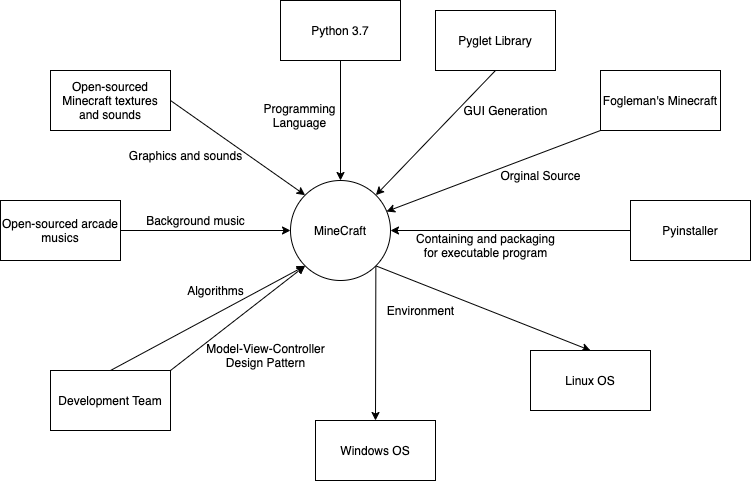
\includegraphics[scale=0.5]{Context.png}
    \caption{\bf{Context Diagram}}
\end{figure}
\FloatBarrier

\subsubsection{Work Partitioning}
\FloatBarrier
\begin{center}
\begin{longtable}[!bpht]{|m{0.3\linewidth}|m{0.35\linewidth}|m{0.35\linewidth}|}\hline
\textbf{Event Name} & \textbf{Input and Output} & \textbf{Summary}\\\hline
Player opens the game & \makecell[ml]{Game Open Request(IN) \\ Game GUI with main\\ menu rendered(OUT)} & \makecell[ml]{The system opens the GUI\\ and loads the main menu\\ when the player requests\\ to open the game}\\\hline

Player opens the game menu & \makecell[ml]{Game Menu Request(IN)\\ Game GUI with game\\ menu rendered(OUT)} & \makecell[ml]{The system updates the\\ GUI and loads the game\\ menu when the player\\ clicks on the game menu\\ button on the main menu}\\\hline

\makecell[ml]{Player opens the\\ setting menu} & \makecell[ml]{Setting Menu Request(IN)\\ Game GUI with setting\\ menu rendered(OUT)} & \makecell[ml]{The system updates the\\ GUI and loads the setting\\ menu when the player\\ clicks on the setting menu\\ button on the main menu}\\\hline

Player quits the game & \makecell[ml]{Game Quit Request(IN)\\ Game GUI closes(OUT)} & \makecell[ml]{The system terminates\\ when the player clicks on\\ the quit button on the\\ main menu}\\\hline

Player starts new game & \makecell[ml]{New Game Request(IN)\\ Game GUI with New \hspace{-0.5mm}Game\\ Scene rendered(OUT)} & \makecell[ml]{The system updates the\\ GUI and loads a new game\\ scene(world) and initialize\\ the game character when\\ the player clicks on the\\ new game button on the\\ game menu}\\\hline

\makecell[ml]{Player starts saved\\ game} & \makecell[tl]{Load Saved Game\\ Request(IN)\\ Saved Game Selection(IN)\\ Game GUI with Saved\\ \hspace{-0.2mm}Game \hspace{-0.5mm}Scene \hspace{-0.5mm}rendered(OUT)} & The system updates the GUI and loads a saved game scene(world) and initialize the game character when the system receives load saved game request and saved game selection\\\hline

\makecell[ml]{Player changes\\ Day-Night Mode} & \makecell[ml]{Day-Night Mode Switch\\ Request(IN) Day-Night\\ Change(OUT)} & \makecell[ml]{The system changes the\\ Day-Night Mode setting\\ when the player requests a\\ Day-Night Mode change on\\ the setting menu or on the\\ ESC menu}\\\hline

\makecell[ml]{Player moves the\\ character} & \makecell[ml]{Movement Keyboard\\ input(IN)\\ Character \hspace{-0.5mm}Movement(OUT)} & \makecell[ml]{The system moves the\\ character according to the\\ movement keyboard input\\ initiated by the player}\\\hline

Player builds a block & \makecell[ml]{Block Build mouse\\ input(IN)\\ Block Type selection\\ keyboard input(IN)\\ New Block(OUT)} & \makecell[ml]{A new block is built by the\\ system at a certain place\\ when the system receives\\Block Build mouse input\\ and Block Type selection\\ keyboard input initiated\\ by the player}\\\hline

Player destroys a block & \makecell[ml]{Block Destroy mouse\\ input(IN)\\ Block Remove(OUT)} & \makecell[ml]{A certain block is\\ destroyed by the system\\ when the system receives\\ Block Destroy mouse input\\ initiated by the player}\\\hline

\makecell[ml]{Player changes the\\ direction of the\\ character} & \makecell[ml]{Direction Change mouse\\ input(IN)\\ New Direction(OUT)} & \makecell[ml]{The system changes the\\ direction of the character\\ when the system receives\\ Direction Change mouse\\ input initiated by the\\ player}\\\hline

\makecell[ml]{Player lets the\\ character jump} & \makecell[ml]{Jump keyboard input(IN)\\ Character Jump(OUT)} & \makecell[ml]{The system lets the\\ character jump when the\\ system receives Jump\\ keyboard input initiated\\ by the player}\\\hline

\makecell[ml]{Player enables the\\ character to fly} & \makecell[ml]{Flying Mode Toggle\\ keyboard input(IN) \\Flying Mode\\ Activation(OUT)} & \makecell[ml]{The system activates the\\ flying mode when the\\ system receives Flying\\ Mode Toggle keyboard\\ input initiated by the\\ player}\\\hline

\makecell[ml]{Player opens the ESC\\ menu} & \makecell[ml]{ESC Menu keyboard\\ input(IN)\\ Game GUI with ESC\\ menu rendered(OUT)} & \makecell[ml]{The system updates the\\ GUI and loads the ESC\\ menu when the system\\ receives ESC Menu\\ keyboard input initiated\\ by the player}\\\hline

\makecell[ml]{Player saves the game\\ scene} & \makecell[ml]{Game Saving Request(IN)\\ Saving Spot Selection(IN)\\ Saved Game Data\\ File(OUT)} & \makecell[ml]{The system saves the game\\ scene when the player\\ requests to save the game\\ and select a saving spot} \\\hline
\caption{\bf{Business Events}}
\end{longtable}
\end{center}
\FloatBarrier
\subsubsection{Individual Product Use Cases(PUC)}

\FloatBarrier
\begin{center}
\begin{longtable}[!bpht]{|m{0.9cm}|m{2.6cm}|m{2.6cm}|m{2.7cm}|m{3.2cm}|m{2.7cm}|}\hline

\textbf{PUC No.} & \textbf{Event Name} & \textbf{Trigger} & \textbf{Preconditions} & \textbf{Procedure} & \textbf{Outcome}\\\hline
1 & \makecell[ml]{Open the\\ game} & \makecell[ml]{The game\\ executable file\\ is clicked} & \makecell[ml]{The game\\ executable is\\ downloaded\\ and installed} & \makecell[ml]{1. The player\\ double left-clicks\\ on the game\\ executable file} & \makecell[ml]{The GUI is\\ loaded with\\ the main menu\\ rendered}\\\hline

2 & \makecell[ml]{Open the\\ game menu} & \makecell[ml]{The game\\ menu button\\ is clicked} & \makecell[ml]{The GUI is at\\ main menu} & \makecell[ml]{1. The player\\ clicks on the game\\\ menu button on\\ the main menu} & \makecell[ml]{The GUI is\\ updated with\\ the game menu\\ rendered}\\\hline

3 & \makecell[ml]{Open the\\ setting menu} & \makecell[ml]{The setting\\ menu button\\ is clicked} & \makecell[ml]{The GUI is at\\ main menu} & \makecell[ml]{1. The player\\ clicks on the\\ setting menu\\ button on the\\ main menu} & \makecell[ml]{The GUI is\\ updated with\\ the setting\\ menu rendered}\\\hline

4 & \makecell[ml]{Quit the game} & \makecell[ml]{The quit\\ button is\\ clicked} & \makecell[ml]{The GUI is at\\ main menu} & \makecell[ml]{1. The player\\ clicks on the quit\\ button on the\\ main menu} & \makecell[ml]{The program\\ terminates and\\ the GUI closes}\\\hline

5 & \makecell[ml]{Start a new\\ game scene} & \makecell[ml]{The new game\\ button is\\ clicked} & \makecell[ml]{The GUI is at\\ game menu} & \makecell[ml]{1. The player\\ clicks on the new\\ game button on\\ the game menu} & \makecell[ml]{The system\\ updates the\\ GUI with a\\ new game\\ scene(world)\\ and initializes\\ the character}\\\hline

6 & \makecell[ml]{Load a saved\\ game scene} & \makecell[ml]{The load\\ game button\\ is clicked} & \makecell[ml]{The GUI is at\\ game menu }& \makecell[ml]{1. The player\\ clicks on the load\\ game button on\\ the game menu\\ 2. The player\\ select a saved\\ game by clicking\\ on the game\\ number button\\(e.g. Game One)} & \makecell[ml]{The system\\ updates the\\ GUI with a\\ saved game\\ scene(world)\\ and initializes\\ the character}\\\hline

7 & \makecell[ml]{Change the\\ Day-Night\\ Mode} & \makecell[ml]{The\\ Day-Night\\ Mode switch\\ is clicked} & \makecell[ml]{The GUI is at\\ setting menu\\ or at ESC menu} & \makecell[ml]{1. The player\\ clicks on\\ Day-Night\\ Mode switch} & \makecell[ml]{The system\\ changes the\\ Day-Night\\ Mode}\\\hline\

8 & \makecell[ml]{Move the\\ character} & \makecell[ml]{The key(s) on\\ the keyboard\\ that controls\\ the movement\\ is pressed} & \makecell[ml]{The game\\ scene(world)\\ is loaded and\\ the character\\ is initialized} & \makecell[ml]{1. The player\\ presses on the\\ movement key on\\ the keyboard} & \makecell[ml]{The system\\ moves the\\ character to a\\ short distance}\\\hline

9 & \makecell[ml]{Build a block} & \makecell[ml]{The key(s) on\\ the keyboard\\ that controls\\ the build type\\ selection and\\ the key on\\ the mouse\\ that controls\\ the build\\ operation are\\ clicked} & \makecell[ml]{The game\\ scene(world)\\ is loaded and\\ the character\\ is initialized} & \makecell[ml]{1. The player\\ presses on the\\ key(s) on the\\ keyboard that\\ controls the build\\ type selection\\ to select a block\\ type to build\\ 2. The player\\ points the\\ crosshair on the\\ surface of a block\\ 3. The player\\ clicks on the key\\ on the mouse\\ that controls the\\ build operation} & \makecell[ml]{The system\\ places a certain\\ type of block\\ next to the one\\ that is pointed\\ to by the\\ crosshair}\\\hline

10 & \makecell[ml]{Destroy a\\ block} & \makecell[ml]{The key on\\ the mouse\\ that controls\\ the destroy\\ operation is\\ clicked} & \makecell[ml]{The game\\ scene(world)\\ is loaded and\\ the character\\ is initialized} & \makecell[ml]{1. The player\\ points the\\ crosshair on\\ the surface of\\ a block that is\\ to be destroyed\\ 2. The player\\ clicks on the key\\ on the mouse\\ that controls the\\ destroy operation} & \makecell[ml]{The system\\ destroys the\\ block that is\\ pointed by the\\ crosshair}\\\hline

11 & \makecell[ml]{Change the\\ direction of\\ the character} & \makecell[ml]{The mouse is\\ moved} & \makecell[ml]{The game\\ scene(world)\\ is loaded and\\ the character\\ is initialized} & \makecell[ml]{1. The player\\ moves the mouse} & \makecell[ml]{The system\\ changes the\\ direction of\\ the character\\ according to\\ the movement\\ of the mouse}\\\hline

12 & \makecell[ml]{Let the\\ character jump} & \makecell[ml]{The key on\\ the keyboard\\ that controls\\ the jump\\ operation is\\ pressed} & \makecell[ml]{The game\\ scene(world)\\ is loaded and\\ the character\\ is initialized} & \makecell[ml]{1. The player\\ presses on the key\\ on the keyboard\\ that controls the\\ jump operation} & \makecell[ml]{The system\\ lets the\\ character jump\\ once}\\\hline

13 & \makecell[ml]{Enable the\\ character to\\ fly} & \makecell[ml]{The key on\\ the keyboard\\ that controls\\ flying mode\\ toggle\hspace{-0.5mm} is\hspace{-0.5mm} clicked} & \makecell[ml]{The game\\ scene(world)\\ is loaded and\\ the character\\ is initialized} & \makecell[ml]{1. The player\\ presses on the key\\ on the keyboard\\ that \hspace{-0.5mm}controls \hspace{-0.5mm}flying\\ mode toggle} & \makecell[ml]{The system\\ activates the\\ flying mode}\\\hline

14 & \makecell[ml]{Open the ESC\\ menu} & \makecell[ml]{\hspace{-0.3mm}The \hspace{-0.5mm}ESC \hspace{-0.5mm}key \hspace{-0.5mm}on\\ the keyboard\\ is clicked} & \makecell[ml]{The game\\ scene(world)\\ is loaded and\\ the character\\ is initialized} & \makecell[ml]{1. The player\\ clicks on the\\ ESC key on the\\ keyboard} & \makecell[ml]{The GUI is\\ loaded with\\ ESC menu\\ rendered} \\\hline

15 & \makecell[ml]{Save the game\\ scene} & \makecell[ml]{The game\\ saving button\\ on the ESC\\ menu is clicked\\ and the game\\ saving spot is\\ selected} & \makecell[ml]{The GUI is at\\ ESC menu} & \makecell[ml]{1. The player\\ clicks on the game\\ saving button on\\ the keyboard\\ 2. The player\\ selects a game\\ saving spot for it} & \makecell[ml]{The system\\ saves the game\\ scene at the\\ selected game\\ saving spot}\\\hline
\caption{\bf{Individual Product Use Cases}}
\end{longtable}
\end{center}
\FloatBarrier
\subsection{Functional Requirements}
\begin{itemize}
        \item \textbf{FR1:} The software game shall start(open the GUI)when the player clicks on the icon of the game.\\
        \textbf{Rationale:} To enable the player to start the game.\\
        \textbf{Criterion:} The player clicks on the icon of the game and the game starts(GUI opens).\\
        \textbf{Related PUC:} 1
        \item \textbf{FR2:} The software game shall load the main menu of the game on the GUI when the game starts.\\
        \textbf{Rationale:} To enable the player to visualize the main menu.\\
        \textbf{Criterion:} The GUI is rendered with the main menu when the game starts.\\
        \textbf{Related PUC:} 1
        \item \textbf{FR2.1:} The main menu should have buttons linked to two sub-menus, game menu and setting menu, the sub-menus should have buttons linked to the main menu.\\
        \textbf{Rationale:} To provide the bidirectional references between the main menu and its sub-menus.\\
        \textbf{Criterion:} The sub-menus can be directed from the main menu and vice versa.\\
        \textbf{Related PUC:} 2,3
        \item \textbf{FR2.1.1:} The game menu should have buttons that support the functionality of playing new game(loading a new game scene) and playing saved game(loading a saved game scene).\\
        \textbf{Rationale:} To provide functionalities of playing new game and playing saved game.\\
        \textbf{Criterion:} The player can start a new game or start a saved game from the game menu.\\
        \textbf{Related PUC:} 5,6
        \item \textbf{FR2.1.2:} The setting menu should support the functionality of Day-Night mode change.\\
        \textbf{Rationale:} To provide the feature of Day-Night Mode.\\
        \textbf{Criterion:} The player can switch the Day-Night Mode on the setting menu.\\
        \textbf{Related PUC:} 7
        \item \textbf{FR2.2:} The main menu should have a button that supports the functionality of game quit and the software game shall terminate(close the GUI) when the player clicks on it.\\
        \textbf{Rationale:} To enable the player to quit the game.\\
        \textbf{Criterion:} The player can quit the game by clicking on the quit game button.\\
        \textbf{Related PUC:} 4
        
        \item \textbf{FR3:} The software game shall load the character of the game on the GUI and place it on the ground when the game scene is loaded.\\
        \textbf{Rationale:} To enable the player to control the character and play the game.\\
        \textbf{Criterion:} The player clicks on start new game button or load saved game button, the character will be initialized on the ground.\\
        \textbf{Related PUC:} 5,6
        
        \item \textbf{FR4:} The GUI shall place a crosshair at the center when the game scene is loaded.\\
        \textbf{Rationale:} To utilize the player with a crosshair, which supports the block build and destroy operation.\\
        \textbf{Criterion:} The player clicks on the icon of the game and can see a crosshair placed at the center of the GUI.\\
        \textbf{Related PUC:} 9,10
        
        \item \textbf{FR4.1:} The crosshair shall be kept at the center of the GUI starting from the game is loaded until the game ends.\\
        \textbf{Rationale:} To ensure the stability of the position of the crosshair.\\
        \textbf{Criterion:} The player plays the game for thirty minutes, the crosshair always keeps its position at the center of the GUI.\\
        \textbf{Related PUC:} 9,10
        
        \item \textbf{FR5:} The software game shall move the character when the player press "W", "A", "S", and "D" keys on the keyboard.\\
        \textbf{Rationale:} To enable the movement of the character.\\
        \textbf{Criterion:} The player clicks on a certain movement key and the character moves accordingly on the GUI.\\
        \textbf{Related PUC:} 8
        
        \item \textbf{FR5.1:} The software game shall move the character forward when the player presses the "W" key on the keyboard.\\
        \textbf{Rationale:} To enable the forward movement of the character.\\
        \textbf{Criterion:} The player clicks on the "W" key on the keyboard and the character moves forward on the GUI.\\
        \textbf{Related PUC:} 8
        
        \item \textbf{FR5.2:} The software game shall move the character to the left when the player presses the "A" key on the keyboard.\\
        \textbf{Rationale:} To enable the left movement of the character.\\
        \textbf{Criterion:} The player clicks on the "A" key on the keyboard and the character moves to the left on the GUI.\\
        \textbf{Related PUC:} 8
        
        \item \textbf{FR5.3:} The software game shall move the character backward when the player presses the "S" key on the keyboard.\\
        \textbf{Rationale:} To enable the backward movement of the character.\\
        \textbf{Criterion:} The player clicks on the "S" key on the keyboard and the character moves backward on the GUI.\\
        \textbf{Related PUC:} 8
        
        \item \textbf{FR5.4:} The software game shall move the character to the right when the player presses the "D" key on the keyboard.\\
        \textbf{Rationale:} To enable the right movement of the character.\\
        \textbf{Criterion:} The player clicks on the "D" key on the keyboard and the character moves to the right on the GUI.\\
        \textbf{Related PUC:} 8
        
        \item \textbf{FR6:} The software game shall change the direction of the character according to the mouse movement controlled by the player.\\
        \textbf{Rationale:} To enable the direction change of the character.\\
        \textbf{Criterion:} The player moves the mouse and the direction of the character changes accordingly.\\
        \textbf{Related PUC:} 11
        
        \item \textbf{FR7:} The software game shall let the character jump when the player presses the space key on the keyboard.\\
        \textbf{Rationale:} To enable the jump action of the character.\\
        \textbf{Criterion:} The player clicks on the space key on the keyboard and the character jumps once.\\
        \textbf{Related PUC:} 12
        
        \item \textbf{FR8:} The software game shall toggle the flying mode when the player presses the tab key on the keyboard.\\
        \textbf{Rationale:} To enable the fly action of the character.\\
        \textbf{Criterion:} The player clicks on the tab key on the keyboard when the flying mode is off. And after that, the player can control the character to fly with "W" and "S" keys on the keyboard.\\
        \textbf{Related PUC:} 13
        
        \item \textbf{FR8.1:} The software game shall enable the flying mode when the flying mode is off and the player presses the tab key on the keyboard.\\
        \textbf{Rationale:} To ensure the correct functionality of the flying mode toggle.\\
        \textbf{Criterion:} The player clicks on the tab key when the flying mode is off, and the flying mode is turned on.\\
        \textbf{Related PUC:} 13
        
        \item \textbf{FR8.2:} The software game shall disable the flying mode when the flying mode is on and the player presses the tab key on the keyboard.\\
        \textbf{Rationale:} To ensure the correct functionality of the flying mode toggle.\\
        \textbf{Criterion:} The player clicks on the tab key when the flying mode is on, and the flying mode is turned off.\\
        \textbf{Related PUC:} 13
        
        \item \textbf{FR8.3:} The software game shall allow the player to control the character to fly using "W" and "S" keys when the flying mode is on.\\
        \textbf{Rationale:} To enable the fly action of the character.\\
        \textbf{Criterion:} The player clicks on the tab key on the keyboard when the flying mode is off. And after that, the player can control the character to fly with "W" and "S" keys on the keyboard.\\
        \textbf{Related PUC:} 13
        
        
        \item \textbf{FR9:} The GUI shall show the outline of a block when the crosshair is pointing to the block.\\
        \textbf{Rationale:} To enable the player to visualize the crosshair's functionality and also to support block build and destroy operations.\\
        \textbf{Criterion:} The player moves mouse to point the crosshair to a block and can see the outline of it.\\
        \textbf{Related PUC:} 9,10,11
        
        \item \textbf{FR10:} The software game shall remove a block when the player moves the mouse to point the crosshair to the block and left-clicks on it.\\
        \textbf{Rationale:} To enable the block destroy operation.\\
        \textbf{Criterion:} The player moves the mouse to point the crosshair to a block and left-clicks on it, the block will be removed.\\
        \textbf{Related PUC:} 10
        
        \item \textbf{FR11:} The software game shall place a new block next to or on the top of an existing block when the player moves the mouse to point the crosshair to the existing block and right-clicks on it.\\
        \textbf{Rationale:} To enable the block build operation.\\
        \textbf{Criterion:} The player moves the mouse to point the crosshair to an existing block and right-clicks on it, the new block will be built.\\
        \textbf{Related PUC:} 9
        
        \item \textbf{FR11.1:} The type of the block to be built shall be changed to the brick type when the player presses "1" on the keyboard.\\
        \textbf{Rationale:} To enable the block type selection.\\
        \textbf{Criterion:} The player clicks on the "1" key on the keyboard and moves the mouse to point the crosshair to an existing block and right-clicks on it, a new brick block will be built.\\
        \textbf{Related PUC:} 9
        
        \item \textbf{FR11.2:} The type of the block to be built shall be changed to the grass type when the player presses "2" on the keyboard.\\
        \textbf{Rationale:} To enable the block type selection.\\
        \textbf{Criterion:} The player clicks on the "2" key on the keyboard and moves the mouse to point the crosshair to an existing block and right-clicks on it, a new grass block will be built.\\
        \textbf{Related PUC:} 9
        
        \item \textbf{FR11.3:} The type of the block to be built shall be changed to the stone type when the player presses "3" on the keyboard.\\
        \textbf{Rationale:} To enable the block type selection.\\
        \textbf{Criterion:} The player clicks on the "3" key on the keyboard and moves the mouse to point the crosshair to an existing block and right-clicks on it, a new stone block will be built.\\
        \textbf{Related PUC:} 9
        
        \item \textbf{FR12:} The software game shall release the mouse movement from the GUI(stop the character direction changing) and show the ESC menu when the player presses "ESC" on the keyboard.\\
        \textbf{Rationale:} To enable the player to visualize the ESC menu.\\
        \textbf{Criterion:} The player clicks on the "ESC" key on the keyboard and the ESC menu will be shown.\\
        \textbf{Related PUC:} 14
        
        
        \item \textbf{FR12.1:} The ESC menu should be able to direct to the game menu.\\
        \textbf{Rationale:} To provide directional reference from ESC menu to the game menu.\\
        \textbf{Criterion:} The player clicks on the save game button on the ESC menu and it directs to the game menu.\\
        \textbf{Related PUC:} 14
        
        
        \item \textbf{FR12.2:} The ESC menu should support the functionalities of Day-Night mode change.\\
        \textbf{Rationale:} To provide the feature of Day-Night Mode.\\
        \textbf{Criterion:} The player can switch the Day-Night Mode on the ESC menu.\\
        \textbf{Related PUC:} 7
        
        \item \textbf{FR12.3:} The ESC menu should support the functionalities of game saving.\\
        \textbf{Rationale:} To enable the player to save the game.\\
        \textbf{Criterion:} The player can save the game on the ESC menu.\\
        \textbf{Related PUC:} 15
        
        \item \textbf{FR13:} The software system shall be able to save up to two game scenes for the player to play at a later time.\\
        \textbf{Rationale:} To provide sufficient capacity for game saving.\\
        \textbf{Criterion:} The player can choose a spot(Game One or Game Two) to save the game on the ESC menu.\\
        \textbf{Related PUC:} 15
        
        \item \textbf{FR14:} The software game shall play the background music when the game starts.\\
        \textbf{Rationale:} To provide more entertainment.\\
        \textbf{Criterion:} The player opens the game and the background music starts to play.\\
        \textbf{Related PUC:} 1
        
        \item \textbf{FR15:} The software game shall play the sound effect when a block is being built or destroyed.\\
        \textbf{Rationale:} To notify the player of the block build or destroy operation.\\
        \textbf{Criterion:} The player destroys or builds a block and should be able to hear the sound effect.\\
        \textbf{Related PUC:} 9,10
        
        \item \textbf{FR16:} The player shall not be able to move through blocks.\\
        \textbf{Rationale:} To ensure the stability of the character movement.\\
        \textbf{Criterion:} The player moves the character to a block and the character should not move through it.\\
        \textbf{Related PUC:} 8
        
        \item \textbf{FR17:} The marble block shall not be built or destroyed.\\
        \textbf{Rationale:} To support the special feature of the marble blocks.\\
        \textbf{Criterion:} The player controls the character to attempt to destroy a marble block and the marble block cannot be destroyed.\\
        \textbf{Related PUC:} 9,10
        
        \item \textbf{FR18:} The keys on the keyboard that are not assigned with any task should not trigger any event to the system or cause the system crash.\\
        \textbf{Rationale:} To avoid the unexpected behaviour of the system caused by trivial keyboard inputs.\\
        \textbf{Criterion:} The player opens the game and start a new game, click on a trivial key and the system does nothing to respond and also does not crash.\\
        \textbf{Related PUC:} 8, 12, 13, 14
\end{itemize}
\section{Non-functional Requirements}

\subsection{Look and Feel Requirements}
\subsubsection{Appearance Requirements}
\begin{itemize}
        \item \textbf{NFR1:} The software game shall be attractive to a teenage player.\\
                    \textbf{Fit Criterion:} \hyperref[s1]{\textbf{Survey 1}} is distributed to the players and the result confirms that the players find the game is attractive to teenage players.
\end{itemize}

\subsection{Usability and Humanity Requirements}
\subsubsection{Ease of Use Requirements}
\begin{itemize}
        \item \textbf{NFR2:} Players aged MIN\_AGE+ shall be able to play the game with no difficulty.\\
        \textbf{Fit Criterion:} \hyperref[s1]{\textbf{Survey 2}} is distributed to the players and the result confirms that the players find that players aged MIN\_AGE+ could play the game with no difficulty.
\end{itemize}
\subsubsection{Personalization and Internationalization Requirements}
\begin{itemize}
        \item None
\end{itemize}
\subsubsection{Learning Requirements}
\begin{itemize}
        \item \textbf{NFR3:} The learning curve of this game shall vary from LEARN\_MIN to LEARN\_MAX minutes depending on the age of the player.\\
        \textbf{Fit Criterion:} \hyperref[s1]{\textbf{Survey 3}} is distributed to the players and the result confirms that the players find that the learning curve of this game varies from LEARN\_MIN to LEARN\_MAX.
\end{itemize}
\subsection{Performance Requirements}
\subsubsection{Speed and Latency Requirements}
\begin{itemize}
        \item \textbf{NFR4:} The response shall be fast enough to avoid interrupting the user's flow of thought.\\
                    \textbf{Fit Criterion:} The software game responds in less than RESPONSE second for 99 percent of the interrogations. No response takes longer than FALSE\_RESPONSE second.
\end{itemize}
\subsubsection{Precision or Accuracy Requirements}
\begin{itemize}
        \item None
\end{itemize}
\subsubsection{Reliability and Availability Requirements}
\begin{itemize}
        \item \textbf{NFR5:} The software game should be available for play HOURS per day, DAYS per year.\\
                    \textbf{Fit Criterion:} 100 times access tests at different time will be applied and the result is 100 successful accesses.
        \item \textbf{NFR6:} The software game shall be able to keep running for a maximum of MAX\_HOUR hours.\\
                    \textbf{Fit Criterion:} A MAX\_HOUR long time program duration test will be applied 3 times and the result is all pass.
\end{itemize}
\subsection{Operational and Environmental Requirements}
\subsubsection{Requirements for Interfacing with Adjacent Systems}
\begin{itemize}
        \item \textbf{NFR7:} The software game shall not perform negative actions on other programs running on the same system.\\
                    \textbf{Fit Criterion:} The software game will be tested with different types of other software programs running and it does not bring negative effects to other programs.
\end{itemize}
\subsection{Maintainability and Support Requirements}
\subsubsection{Maintenance Requirements}
\begin{itemize}
        \item \textbf{NFR8:} An update must be applied to the software game when a bug is revealed.\\
                    \textbf{Fit Criterion:} Every time there is a bug revealed, the team updates the product.
\end{itemize}
\subsubsection{Supportability Requirements}
\begin{itemize}
        \item None
\end{itemize}
\subsubsection{Adaptability Requirements}
\begin{itemize}
        \item \textbf{NFR9:} The software game shall be able to run on Windows and Linux OS.\\
                    \textbf{Fit Criterion:} The software game will be tested on both a Windows OS and a Linux OS and the test cases all pass.
\end{itemize}
\subsection{Security Requirements}
\subsubsection{Integrity Requirements}
\begin{itemize}
        \item \textbf{NFR10:} The software game shall protect itself from intentional abuse.\\
                    \textbf{Fit Criterion:} Specific threat test cases will be made and the threats are prevented.
\end{itemize}
\subsubsection{Privacy Requirements}
\begin{itemize}
        \item None
\end{itemize}
\subsection{Cultural Requirements}
\subsubsection{Cultural Requirements}
\begin{itemize}
        \item \textbf{NFR11:} The software game shall not be offensive to any religious or ethic groups.\\
        \textbf{Fit Criterion:} \hyperref[s1]{\textbf{Survey 4}} is distributed to the players and the result confirms that the players find that this game is not offensive to any religious or ethic group.
\end{itemize}
\subsubsection{Political Requirements}
\begin{itemize}
        \item None
\end{itemize}
\subsection{Legal Requirements}
\subsubsection{Compliance Requirements}
\begin{itemize}
        \item \textbf{NFR12:} The product shall not violate the Digital Millennium Copyright Act\cite{act}.\\
        \textbf{Fit Criterion:} A legal expert will be asked to check if this game confirms the Digital Millennium Copyright Act and the result is meeting.
\end{itemize}
\subsection{Health and Safety Requirements}
\begin{itemize}
        \item \textbf{NFR13:} The product shall not generate any mental or physical threat to the safety of the players.\\
        \textbf{Fit Criterion:} A safety domain expert will be asked to check if this game meets the safety standard and the result is meeting.
\end{itemize}
\subsection{Robustness Requirements}
\begin{itemize}
        \item \textbf{NFR14:} Any key with no task assigned should not trigger any event to the system.\\
        \textbf{Fit Criterion:} The tester opens the game and clicks on a key on the keyboard that is not assigned any task, nothing happens to the system and the system does not crash.\\
\end{itemize}
\section{Project Issues}

\subsection{Open Issues}
Our investigation into whether Pyglet is the best fit GUI library for the design of this game product is still an open issue.
\subsection{Off-the-Shelf Solutions}
The original project designed and developed by Folgleman \cite{mine} will be considered as the candidate component for the development of this software game. Online open-source Minecraft textures and sounds will be considered as source elements to create graphics and sounds of the game.
\subsection{New Problems}
One potential problem of this software game could be that the player feels it is too similar to the well-known Minecraft game released by Microsoft. Another problem is that the further development for game features extension could be difficult due to the limitation of Pyglet.
\subsection{Tasks}
The project development plan can be found \href{https://gitlab.cas.mcmaster.ca/wangs132/minecraft/blob/master/Doc/DevelopmentPlan/DevelopmentPlan.pdf}{\textbf{HERE}}.
\subsection{Migration to the New Product}
None
\subsection{Risks}
Due to time constraints, the development team might not be able to fully learn all the functionalities provides by Pyglet. Therefore, some features that are planned out might not be able to be fully implemented according to this requirement specification. This document will be revised in the case that some features or functionalities need to be removed.
\subsection{Costs}
Since all the sources(including textures, sounds, original program) and tools(including Python, Pyglet, Pyinstaller) are open-source, there will be no monetary cost for the development. The time cost of the development will be 3 months.
\subsection{User Documentation and Training}
A beginner's manual, also called \href{https://gitlab.cas.mcmaster.ca/wangs132/minecraft/-/blob/master/Doc/UserGuide/UserGuide.pdf}{ \bf User Guide} will be added to the project as a guideline of how to install and play the game. The beginning manual will include all the basic operations that the player could do. With the help of the manual, the player will be able to learn the game.
\subsection{Waiting Room}
The toolbox feature is still under consideration.
\subsection{Ideas for Solutions}
None
\bibliographystyle{plainnat}

\bibliography{SRS}

\newpage

\section{Appendix}

\subsection{NFR Surveys}


\begin{itemize}
        \item \textbf{Survey 1:}\label{s1} The survey will ask for the attractiveness(a rank between 1-10), the average of the result should be above \textbf{AVG1} to pass the test.
        \item \textbf{Survey 2:}\label{s2} The survey will ask for the difficulty of the game(a rank between 1-10), the average of the result should be below \textbf{AVG2} to pass this test.
        \item \textbf{Survey 3:}\label{s3} The survey will ask for the learning time of the game, the average of the result should be between \textbf{LEARN\_MIN} to \textbf{LEARN\_MAX} minutes to pass this test.
        \item \textbf{Survey 4:}\label{s4}  The survey will ask for the satisfaction of the cultural politeness of the game(a rank between 1-10), the average of the result should be above \textbf{AVG1} to pass this test.
\end{itemize}

\subsection{Symbolic Parameters}


\begin{itemize}
    \item \textbf{MIN\_AGE: 7}
    \item \textbf{HOURS: 24}
    \item \textbf{DAYS: 365}
    \item \textbf{MAX\_HOUR: 10}
    \item \textbf{AVG1: 7}
    \item \textbf{AVG2: 3}
    \item \textbf{LEARN\_MIN: 2}
    \item \textbf{LEARN\_MAX: 30}
    \item \textbf{RESPONSE: 0.1}
    \item \textbf{FALSE\_RESPONSE: 0.5}
\end{itemize}

\newpage
\begin{thebibliography}{9}
\bibitem{mine} 
Fogleman, “fogleman/Minecraft,” 
        GitHub, 16-Feb-2019. [Online]. Available: 
        https://github.com/fogleman/Minecraft. [Accessed: 
        10-Feb-2020].
\bibitem{act} 
”Video Games and the law: Copyright, 
        Trademark and Intellectual Property”, NewMediaRights, 2020. [Online]. 
        Available: https://www.newmediarights.org/guide/legal/Video\_Games\_law\_
        Copyright\_Trademark\_Intellectual\_Property. [Accessed: 06- Feb- 
        2020].
\end{thebibliography}
\end{document}